\documentclass[varwidth, border=10pt]{standalone}
\usepackage{tikz}
\usetikzlibrary{shapes.geometric}    % trapezium
\usetikzlibrary{arrows}              % arrow tips
\usepackage{amsmath}
\usepackage{bm}                      % boldsymbol
\usepackage{makecell}                % makecell
\usetikzlibrary{matrix,calc}
\usepackage{color}
\usepackage{xcolor}
\definecolor{mygray}{HTML}{F0F0F0}

\begin{document}
\begin{figure}
  \begin{minipage}{0.36\linewidth}
    \centering
    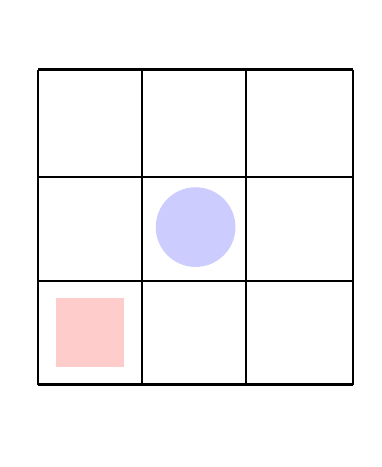
\begin{tikzpicture}[baseline=0, >=latex',thick, scale=0.8, every node/.style={scale=0.8}]]
      % states
      \coordinate (center) at (0,0);
      \coordinate (xlength) at (5, 0);
      \coordinate (ylength) at (0, 5);

      \node [circle, name=buttom_left] at
      ($(center) + (ylength) + (0, 0.5)$) {};
      \node [circle, name=bottom_right] at
      ($(center) + (0, -0.7)$) {};

      \draw [-] (center) -- ($(xlength)$);
      \draw [-] (center) -- ($(ylength)$);
      \draw [-] ($(ylength)$) -- ($(xlength) + (ylength)$);
      \draw [-] ($(xlength) + (ylength)$) -- ($(xlength)$);

      \draw [-] ($(center) + 0.33*(xlength)$) -- ($(center) + 0.33*(xlength) + (ylength)$);
      \draw [-] ($(center) + 0.66*(xlength)$) -- ($(center) + 0.66*(xlength) + (ylength)$);
      \draw [-] ($(center) + 0.33*(ylength)$) -- ($(center) + 0.33*(ylength) + (xlength)$);
      \draw [-] ($(center) + 0.66*(ylength)$) -- ($(center) + 0.66*(ylength) + (xlength)$);

      \node [draw=blue!20, circle, fill=blue!20, minimum size=35pt] at ($(center) +
      0.5*(xlength) + 0.5*(ylength)$) {};
      \node [draw=red!20, rectangle, fill=red!20, minimum size=30pt] at
      ($(center) + 0.5*0.33*(xlength) + 0.5*0.33*(ylength)$) {};
    \end{tikzpicture}~\\
    \textbf{image}
  \end{minipage}
  \begin{minipage}{0.17\linewidth}
    \centering
    \Large{
      $\stackrel{\text{image parser}}{\Longrightarrow}$}
  \end{minipage}
  \begin{minipage}{0.45\linewidth}
    \centering
    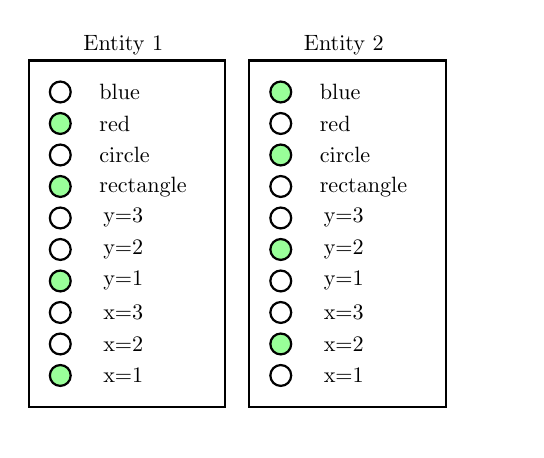
\begin{tikzpicture}[>=latex',thick, scale=0.8, every node/.style={scale=0.8}]]
      % states
      \coordinate (center) at (0,0);
      \coordinate (xlength) at (5, 0);
      \coordinate (ylength) at (0, 5);

      \node [circle, name=buttom_left] at
      ($(center) + (ylength) + (0, 0.5)$) {};
      \node [circle, name=bottom_right] at
      ($(center) + (0, -0.5)$) {};

      \coordinate (newcenter) at (0, -0.8);
      \coordinate (ydistance) at (0, 1);
      \coordinate (xdistance) at (1, 0);


      % entity 1: red rectangle
      \node [name=c1, draw, fill=green!40, circle, minimum size=5pt] at
      ($(newcenter) + (ydistance)$) {};
      \node [right of=c1] {\textcolor{white}{}x=1};
      \node [draw, circle, minimum size=5pt, name=c2] at
      ($(newcenter) + 1.5*(ydistance)$) {};
      \node [right of=c2] {\textcolor{white}{}x=2};
      \node [draw, circle, minimum size=5pt, name=c3] at
      ($(newcenter) + 2*(ydistance)$) {};
      \node [right of=c3] {\textcolor{white}{}x=3};
      \node [draw, fill=green!40, circle, minimum size=5pt, name=c4] at
      ($(newcenter) + 2.5*(ydistance)$) {};
      \node [right of=c4] {\textcolor{white}{}y=1};
      \node [draw, circle, minimum size=5pt, name=c5] at
      ($(newcenter) + 3*(ydistance)$) {};
      \node [right of=c5] {\textcolor{white}{}y=2};
      \node [draw, circle, minimum size=5pt, name=c6] at
      ($(newcenter) + 3.5*(ydistance)$) {};
      \node [right of=c6] {\textcolor{white}{}y=3};
      \node [draw, fill=green!40, circle, minimum size=5pt, name=c7] at
      ($(newcenter) + 4*(ydistance)$) {};
      \node [text width=3cm] at ($(c7) + (2.12,0)$) {\textcolor{white}{}rectangle};
      \node [draw, circle, minimum size=5pt, name=c8] at
      ($(newcenter) + 4.5*(ydistance)$) {};
      \node [text width=3cm] at ($(c8) + (2.12,0)$) {\textcolor{white}{}circle};
      \node [draw, circle, minimum size=5pt, name=c9, fill=green!40] at
      ($(newcenter) + 5*(ydistance)$) {};
      \node [text width=3cm] at ($(c9) + (2.12,0)$) {\textcolor{white}{}red};
      \node [draw, circle, minimum size=5pt, name=c10] at
      ($(newcenter) + 5.5*(ydistance)$) {};
      \node [text width=3cm, name=c11] at ($(c10) + (2.12,0)$) {\textcolor{white}{}blue};

      \draw ($(c1) + (-0.5, -0.5)$) rectangle ($(c11) + (0.5, 0.5)$);
      \node at ($(c1) + (1, 5.25)$) {Entity 1};

      % entity 2
      \node [name=b1, draw, circle, minimum size=5pt] at
      ($(newcenter) + 3.5*(xdistance) + (ydistance)$) {};
      \node [right of=b1] {\textcolor{white}{}x=1};
      \node [draw, circle, fill=green!40, minimum size=5pt, name=b2] at
      ($(newcenter) + 3.5*(xdistance) + 1.5*(ydistance)$) {};
      \node [right of=b2] {\textcolor{white}{}x=2};
      \node [draw, circle, minimum size=5pt, name=b3] at
      ($(newcenter) + 3.5*(xdistance) + 2*(ydistance)$) {};
      \node [right of=b3] {\textcolor{white}{}x=3};
      \node [draw, circle, minimum size=5pt, name=b4] at
      ($(newcenter) + 3.5*(xdistance) + 2.5*(ydistance)$) {};
      \node [right of=b4] {\textcolor{white}{}y=1};
      \node [draw, circle, fill=green!40, minimum size=5pt, name=b5] at
      ($(newcenter) + 3.5*(xdistance) + 3*(ydistance)$) {};
      \node [right of=b5] {\textcolor{white}{}y=2};
      \node [draw, circle, minimum size=5pt, name=b6] at
      ($(newcenter) + 3.5*(xdistance) +3.5*(ydistance)$) {};
      \node [right of=b6] {\textcolor{white}{}y=3};
      \node [draw, circle, minimum size=5pt, name=b7] at
      ($(newcenter) + 3.5*(xdistance) +4*(ydistance)$) {};
      \node [text width=3cm] at ($(b7) + (2.12,0)$) {\textcolor{white}{}rectangle};
      \node [draw, circle, minimum size=5pt, fill=green!40, name=b8] at
      ($(newcenter) + 3.5*(xdistance)+ 4.5*(ydistance)$) {};
      \node [text width=3cm] at ($(b8) + (2.12,0)$) {\textcolor{white}{}circle};
      \node [draw, circle, minimum size=5pt, name=b9] at
      ($(newcenter) + 3.5*(xdistance) + 5*(ydistance)$) {};
      \node [text width=3cm] at ($(b9) + (2.12,0)$) {\textcolor{white}{}red};
      \node [draw, circle, minimum size=5pt, name=b10, fill=green!40] at
      ($(newcenter) + 3.5*(xdistance) + 5.5*(ydistance)$) {};
      \node [text width=3cm, name=b11] at ($(b10) + (2.12,0)$) {\textcolor{white}{}blue};

      \draw ($(b1) + (-0.5, -0.5)$) rectangle  ($(b11) + (0.5, 0.5)$);
      \node at ($(b1) + (1, 5.25)$) {Entity 2};

      % \draw [white, -] ($(center) + (0, 0.3)$) -- ($1.17*(ylength)$);
    \end{tikzpicture}~\\
    \textbf{state representation}
  \end{minipage}
\end{figure}
\end{document}